%%% Modelo de Lista de Exercícios para Universidade
%%% Criado por Diogo Roberto R. Freitas (diogo@poli.br)
%%% Livre para alterações
\documentclass[12pt,onepage,a4paper]{memoir}

%% Language and font encodings
\usepackage[english,portuges]{babel}
\usepackage[T1]{fontenc}
\usepackage[utf8]{inputenc}

%% Sets page size and margins
\usepackage[a4paper,top=2.5cm,bottom=2cm,left=2cm,right=2cm,marginparwidth=1.75cm]{geometry}
\setlength\parindent{0cm} % Tamanho da tabulação dos parágrafos

%%% ATENÇÃO!!! %%%
%%% Preencha estes comandos com suas informações
\newcommand{\logo}{
\includegraphics[width=0.4\textwidth]{univasf.jpg}} % inclua o arquivo com o logo da instituição
\newcommand{\univ}{Univasf - Salgueiro/PE}
%\newcommand{\escola}{Escola Politécnica de Pernambuco}
\newcommand{\disc}{Rede de Computadores}
\newcommand{\auth}{Prof. Marcos Bião}
\newcommand{\email}{\url{marcos.biao@univasf.edu.br}}
%\newcommand{\sitedisc}{\url{canvas.instructure.com/courses/1139439}} % site da disciplina
\newcommand{\cabec}{Univasf - Salgueiro/PE} % cabeçalho a partir da 2ª página
\newcommand{\tit}{Lista de exercícios}    


%%%%%%%%%

%% Useful packages
\usepackage{amsmath}
\usepackage{graphicx}
\usepackage[colorinlistoftodos]{todonotes}
\usepackage[colorlinks=true, allcolors=blue]{hyperref}
\linespread{1.25}
\usepackage{graphicx}
\usepackage{nicefrac}
\usepackage[tight]{units}
\usepackage[justification=centering]{caption}
\usepackage{subcaption}
\usepackage{lastpage}
\usepackage{pstricks}
\usepackage{url}% ou hyperref
%\usepackage{breakurl}
\usepackage{multirow}
\usepackage{tabulary}
\usepackage{longtable}
\usepackage{microtype}% improves the spacing between words and letters
\usepackage{booktabs}%  helps you improve the quality of your LaTeX tables
\usepackage{rotfloat}
\usepackage{rotating}
\usepackage{amsmath}
\usepackage{multicol}%multiplas colunas

\usepackage{listings}

%%% NÃO ALTERAR ESTES COMANDOS 
%%% Configura a primeira página
\makepagestyle{1pagina}
\makeoddhead{1pagina}{
	\logo \\
    \vspace{5pt}
    %\textsf{\univ \\ \escola \\} %%% Caso o logo não tenha o nome da universidade descomente essa linha
    \textsf{Disciplina: \disc \\
	\auth~(\email) \\
    Última atualização: \today
    \sitedisc }
    }{}{}
\makeoddfoot{1pagina}{\tiny Documento produzido em \LaTeX}{}{\scriptsize Página \thepage~de \thelastpage}
\makefootrule{1pagina}{\textwidth}{\normalrulethickness}{5pt}
%%% Configura as demais páginas
\makepagestyle{paginacomum}
\makeevenhead{paginacomum}{\textsf{\scriptsize \cabec~-- \auth}}{}{}
\makeevenfoot{paginacomum}{\tiny Documento produzido em \LaTeX}{}{\scriptsize Página \thepage~de \thelastpage}
\makeoddhead{paginacomum}{\textsf{\scriptsize \cabec~-- \auth}}{}{}
\makeoddfoot{paginacomum}{\tiny Documento produzido em \LaTeX}{}{\scriptsize Página \thepage~de \thelastpage}
\makeheadrule{paginacomum}{\textwidth}{\normalrulethickness}
\makefootrule{paginacomum}{\textwidth}{\normalrulethickness}{5pt}
\pagestyle{paginacomum}
%%%


%%% Início do documento
\begin{document}
\thispagestyle{1pagina}
\vspace*{3.5cm} %%% Caso o cabeçalho cubra estes texto aumente o "vspace"
\begin{center}
    \textbf{\textsf{\large \tit}} %%% não altere aqui
\end{center}
\newcounter{cont}
\begin{center}
    \textbf{Introdução}
\end{center}

\begin{enumerate} % início das questões, pode escrever aqui
% Questão 1

    \item \label{a1}Faça as conversões de base pedidas, mostrando as divisões/multiplicações efetuadas, caso sejam necessárias:
    \begin{multicols}{2}
        \begin{enumerate}
            \item $15_{10}$ para binário
            \item $43_{10}$ para binário
            \item $83_{10}$ para binário
            \item $128_{10}$ para binário
            \item $15_{10}$ para hexadecimal
            \item $43_{10}$ para hexadecimal
            \item $83_{10}$ para hexadecimal
            \item $128_{10}$ para hexadecimal
        \end{enumerate}
    \end{multicols}

    \item Faça as conversões de base pedidas, mostrando as divisões/multiplicações efetuadas, caso sejam necessárias:
    \begin{multicols}{2}
        \begin{enumerate}
            \item $1010_{2}$ para decimal
            \item $1111_{2}$ para decimal
            \item $101101_{2}$ para decimal
            \item $110011_{2}$ para decimal
            \item $1010_{2}$ para hexadecimal
            \item $1111_{2}$ para hexadecimal
            \item $101101_{2}$ para hexadecimal
            \item $110011_{2}$ para hexadecimal
        \end{enumerate}
    \end{multicols}    

    \item Faça as conversões de base pedidas, mostrando as divisões/multiplicações efetuadas, caso sejam necessárias:
    \begin{multicols}{2}
    \begin{enumerate}
        \item $479_{16}$ para decimal
        \item $4AB_{16}$ para decimal
        \item $BDE_{16}$ para decimal
        \item $F0CA_{16}$ para decimal
        \item $2D3F_{16}$ para decimal
        \item $84_{16}$ para binário
        \item $7F_{16}$ para binário
        \item $3B8C_{16}$ para binário
        \item $47FD_{16}$ para binário
        \item $F1CD_{16}$ para binário
    \end{enumerate}
    \end{multicols}
    
     \item Determine o resultado das seguintes operações aritméticas binárias.
     \begin{multicols}{2}
        \begin{enumerate}
            \item 110101 + 11001
            \item 101110 + 100101
            \item 1110010 + 1101101
            \item 101 + 100101
            \item 1110 + 1001011 + 11101
            \item 101110 - 100101
            \item 1100 - 1010
            \item 11011101 - 1100011
            \item 11110 - 1111
            \item 1011001 - 11011
            \item 100000 - 11100
            \item 10101 x 11
            \item 11001 x 101
            \item 110110 x 111
            \item 11110 x 110
        \end{enumerate}
    \end{multicols}    
           

    \item Indique se ocorre ou não overflow ao efetuar as seguintes adições de operandos com 8 bits.
        \begin{enumerate}
            \item 11010100 + 10101011
            \item 10111001 + 11010110
            \item 01011101 + 00100001
            \item 00100110 + 01011010
        \end{enumerate}

    \item Indique a gama de valores decimais que se podem representar em binário com 4 bits usando a representação em sinal e grandeza.

    \item Represente os números $+97_{10} $  e  $ -121_{10}$, usando representação binária com sinal.

    \item Considere duas variáveis lógicas, C – que indica se chove – e F – que indica se faz frio, e as funções lógicas abaixo:
    \begin{itemize}
        \item P – o tempo está péssimo quando chove e faz frio;
        \item R – o tempo está ruim quando chove ou faz frio;
        \item M – o tempo está mais ou menos quando chove mas não faz frio, ou vice-versa;
        \item B – o tempo está bom quando não chove nem está frio;
        \item S – o tempo está seco quando não chove.
    \end{itemize}

    Complete as tabelas verdades a seguir, onde 1 representa \textit{verdadeiro} e 0 representa \textit{falso}.

    \begin{table}[H]
    \centering
\begin{tabular}{|ll|l|l|l|l|l|}
\hline
C & F & P & R & M & B & S \\ \hline
0 & 0 &   &   &   &   &   \\ \cline{3-7} 
1 & 1 &   &   &   &   &   \\ \cline{3-7} 
0 & 0 &   &   &   &   &   \\ \cline{3-7} 
1 & 0 &   &   &   &   &   \\ \hline
\end{tabular}
\end{table}

    \item Determine a expressão final do circuito a seguir:
    \begin{figure}[H]
        \centering
        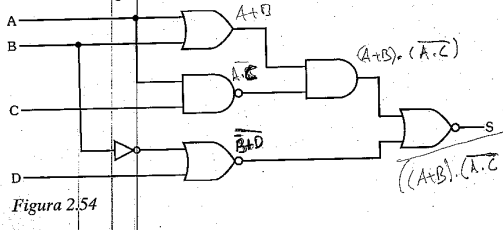
\includegraphics[scale=0.65]{fig/circuito.png}
        \label{fig:circuitoExpressao01}
    \end{figure}


    \item Escreva a tabela verdade de cada uma das expressões a seguir:
    \begin{enumerate}
        \item F = $X+\overline{Y+Z}$
        \item F = $X\overline{(Y+Z)}+XY$
        \item F = $\overline{\overline{X}+Y+Z}$
        \item F =  $(\overline{A}+B+C)(A+\overline{B}+\overline{D})(B+\overline{C}+\overline{D})(A+B+C+D)$
        \item F = $(A+\overline{A})B+AB\overline{C}+C(A+\overline{B})(\overline{A}+B)$
    \end{enumerate}

    \item Desenhe o circuito lógico para as seguintes expressões:
    \begin{enumerate}
        \item $F = (A+B).(C+D)$
        \item $F = A.B+\overline{C}+(\overline{CD})$
        \item $F = [\overline{\overline{A}.B(\overline{B.C}).(\overline{B+D})}]$
        \item $F = [(\overline{\overline{\overline{A}.B}+(\overline{A.\overline{B}})+\overline{C}})].(C+D)$
        \item $F = \overline{A}.[\overline{\overline{B}.C+A.(\overline{C+\overline{D}})+B.\overline{C}.D}]+B.\overline{D}$
        \item $F = \overline{C}.[\overline{A.\overline{B}+B.(\overline{A}+C)}]$
    \end{enumerate}

    
    \item Escreva uma expressão booleana para as funções lógicas representadas pelas tabelas de verdade.
    
    \begin{enumerate}
        \item  .
                \begin{table}[H]
                    \begin{tabular}{|l|l|l|}
                    \hline
                        x & y & f \\ \hline
                        0 & 0 & 1 \\ \hline
                        0 & 1 & 0 \\ \hline
                        1 & 0 & 0 \\ \hline
                        1 & 1 & 1 \\ \hline
                    \end{tabular}
                \end{table}

        \item .
                \begin{table}[H]
\begin{tabular}{|l|l|l|l|}
\hline
x & y & z & f \\ \hline
0 & 0 & 0 & 0 \\ \hline
0 & 0 & 1 & 1 \\ \hline
0 & 1 & 0 & 0 \\ \hline
0 & 1 & 1 & 0 \\ \hline
1 & 0 & 0 & 1 \\ \hline
1 & 0 & 1 & 0 \\ \hline
1 & 1 & 0 & 1 \\ \hline
1 & 1 & 1 & 0 \\ \hline
\end{tabular}
\end{table}
    \end{enumerate}
       
    \item Obtenha a tabela de verdade para cada uma das funções.
    \begin{enumerate}
        \item $F = \overline{X}Y + \overline{XY}Z$
        \item $F = \overline{WX}\overline{(\overline{Y} + \overline{Z})}$
        \item $F = (\overline{A} + B + C)(A + \overline{B} + \overline{D})(B + \overline{C} + \overline{D})(A + B + C + D)$
        \item $F = (A + \overline{A})B + BA\overline{C} + C(A + \overline{B})(\overline{A} + B)$
    \end{enumerate}

    \item Complete cada expressão:
    \begin{multicols}{2}
    \begin{enumerate}
        \item $X + 1 =$ 
        \item $X + 0 =$
        \item $X + X =$
        \item $X.X =$ 
        \item $X.0 =$ 
        \item $X.\overline{X} =$
        \item $X + \overline{X} =$
        \item $X.1 =$ 
        \item $X + 0 =$
        \item $X + \overline{X} =$ 
        \item $X + XY =$ 
        \item $Y +\overline{X}.Y =$
    \end{enumerate}
    \end{multicols}

    \item Use os teoremas da álgebra de Boole para simplificar as seguintes funções booleanas.
    \begin{enumerate}
        \item $F = \overline{A}B+ A\overline{B} + AB$
        \item $F = ABC + A\overline{C} + A\overline{B}$
        \item $F = (AB\overline{C})(\overline{A} + \overline{B} + \overline{C})$
        \item $F = \overline{X}(X+Y)+\overline{Z}+YZ$
        \item $F = (A+\overline{B}+AB).(A+\overline{B})(\overline{A}.B)$
        \item $F = (A+B+C)(\overline{A}+\overline{B}+C)$
        \item $F = WXYZ(WXY\overline{W} + W\overline{X}YZ + \overline{W}XYZ + WX\overline{Y}Z)$
        \item $F = AB + AB\overline{C}D + ABD\overline{E} + AB\overline{C}E + \overline{C}DE$
        \item $F = MNO + \overline{Q}P\overline{N} + PRM + \overline{Q}OM\overline{P} + MR$
        \item $F = \overline{A}.\overline{B}.C+ \overline{A}.B.C+\overline{A}.B.\overline{C}+A.B.C + A.B.\overline{C}$
    \end{enumerate}

    \item Aplicar os Teoremas de Morgan nos seguintes casos:
    \begin{enumerate}
        \item $F = \overline{A(B+C)}$
        \item $F = \overline{\overline{AB+CD}.E}$
        \item $F = \overline{(AB+CD)E}$
        \item $F = \overline{(\overline{AC}+ B+D)} + C(\overline{ACD})$
        \item $F = [\overline{(A+B)C}]+[\overline{D(C+B)}]$
        \item $F = [\overline{\overline{X}.\overline{Y}.\overline{Z}.(X+Y+\overline{Z}}]$
    \end{enumerate}

    \item Simplifique as expressões a seguir utilizando o mapa de karnaugh
    \begin{enumerate}
        \item $F=\overline{A}.\overline{B}.\overline{C} + \overline{A}.\overline{B}.C+AB.\overline{C}+A.\overline{B}.\overline{C}$
        \item $F = \overline{A}.\overline{B}.C+\overline{A}.B.\overline{C}+A.B\overline{C}+A.B.C$
        \item $F = A.B.C.D+A.B.\overline{C}.D+A.B.\overline{C}.\overline{D}+A.\overline{B}.C.D+\overline{A}.B.C.D+\overline{A}.B.C.\overline{D}+\overline{A}.B.\overline{C}.D+\overline{A}.\overline{B}.\overline{C}.D$
    \end{enumerate}

\begin{center}
    \textbf{Projeto de circuitos}
\end{center}

    \item Projete um circuito lógico cuja saída seja nível lógico ALTO apenas quando a maioria das entradas A, B e C for nível lógico BAIXO.

    \item O circuito recebe dois números binários de dois bits, A e B. Projete um circuito para produzir a saída quando A > B.

    \item Projete um circuito que receberá um número binário de quatro bits e indicará quando o número é divisível por 2, 5 e 6.

    \item Quatro juízes participam de um programa de televisão e cada um tem, a sua disposição, uma chave on/off correspondente ao julgamento de um calouro (on – aprovado, off – reprovado). Na saída temos três lâmpadas, correspondentes a três resultados: aprovado (pela maioria), reprovado (pela maioria) e empate. Desenvolva um circuito lógico.

    \item Uma fabrica precisa de uma sirene para indicar o fim do expediente. A sirene deve ser ativada quando ocorrer uma das seguintes condições:
    \begin{itemize}
        \item Já passou das 17h e todas as máquinas estão desligadas.
        \item É sexta-feira, a produção do dia foi atingida e todas as máquinas estão paradas.
    \end{itemize}
    Projete um circuito lógico para o funcionamento da sirene.

    \item Um número de 4 bits que é representado por $A_{3}A_{2}A_{1}A_{0}$, sendo $A_{0}$ o bit menos significativo. Projete um circuito lógico que gere uma saída em nível ALTO sempre que o número binário for maior que 0010 e menor que 1000. 

    \item A figura seguinte mostra um sistema de alarme usado para sinalizar ao condutor de um automóvel certas situações. Os três interruptores são usados para indicar o estado da porta do condutor, o estado da ignição e o estado das luzes. Projete o circuito de controlo do alarme de modo que este só seja ativado nas seguintes condições:
    \begin{itemize}
        \item As luzes estão ligadas enquanto a ignição está desligada;
        \item A porta está aberta enquanto a ignição está ligada.
    \end{itemize}

    \begin{figure}[H]
        \centering
        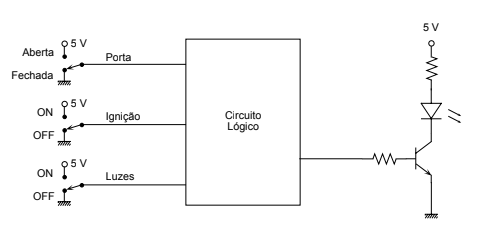
\includegraphics[scale=0.6]{fig/ignicao.png}
        \label{fig:ignicao}
    \end{figure}


    \item A figura que se segue mostra parte do sistema de controlo de uma fotocopiadora. Os interruptores S1, S2, S3 e S4 encontram-se distribuídos por vários pontos de passagem do papel pela máquina. O estado deles é normalmente aberto, só fechando quando o papel passa por eles. Devido à distância entre eles, S1 e S4 nunca podem estar fechados ao mesmo tempo. Projete o circuito lógico que produz um sinal ativo alto na saída X sempre que dois ou mais interruptores estão fechados.

    \begin{figure}[H]
        \centering
        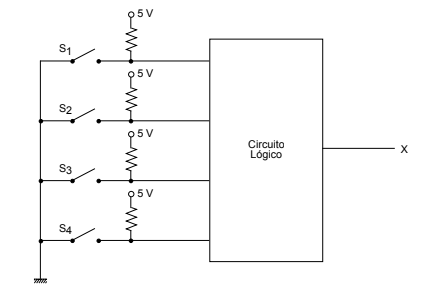
\includegraphics[scale=0.6]{fig/copiadora.png}
        \label{fig:copiadora}
    \end{figure}

    \item Projete um circuito lógico de uma porta de elevador em um prédio de 3 andares. M indica movimento; F1, F2, F3 indicadores de andares e são normalmente nível baixo e passa para nível alto apenas quando estiver no andar. A saída do circuito é o sinal de ABRIR a porta que normalmente é nível BAIXO. Se acionado para abrir a porta, sobe para ALTO.

    \begin{figure}[H]
        \centering
        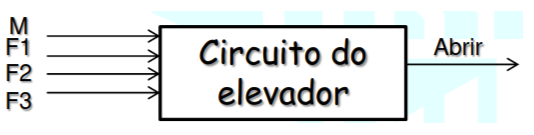
\includegraphics[scale=0.6]{fig/elevador.png}
        \label{fig:elevador}
    \end{figure}

    \item Um misturador de tintas está representado pela figura a seguir. Neste sistema temos o motor que gira a hélice que mistura a tinta, representado pela letra M, o sensor de nível A, que indica que o nível do tanque já atingiu o valor mínimo para que o motor comece a funcionar. Temos também as válvulas que permitem a passagem das tintas, representadas pelas letras B, C e D. Tanto o motor, quanto o sensor e as válvulas são considerados ligados ou ativados quando estiverem com nível lógico 1 e desligados ou desativados quando estiverem com nível lógico 0. Projete um circuito digital para controle do motor M para que somente quando o nível do tanque atingir o sensor A e duas ou mais válvulas estiverem acionadas. Monte a tabela verdade e obtenha a expressão reduzida utilizando o Mapa de Karnaugh. Desenhe o circuito resultante.

    \begin{figure}[H]
        \centering
        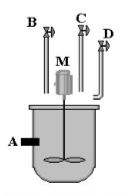
\includegraphics[scale=0.6]{fig/misturador.png}
        \label{fig:misturador}
    \end{figure}

    \item O sistema abaixo é composto por quatro fornos (A,B,C,e D). Cada forno tem um controlador de temperatura (CA,CB,CC,e CD), que faz o controle da temperatura no respectivo forno. Se a temperatura de determinado forno ultrapassar um valor programado no controlador, o respectivo alarme é ativado. No caso, quando algum dos controladores estiver com seu respectivo alarme ligado a saída correspondente (A,B,C e D) tem nível lógico 1, caso contrário, tem nível lógico 0. Projete um circuito digital que ative o SINALIZADOR sempre que dois ou três saídas de alarmes estiverem ativos, em qualquer outra situação o SINALIZADOR deverá estar desligado. Monte a tabela verdade e simplifique a expressão utilizando o Mapa de Karnaugh. Desenhe o circuito resultante.

    \begin{figure}[H]
        \centering
        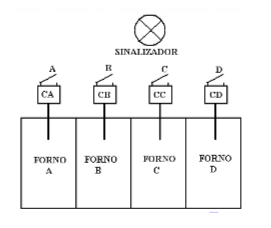
\includegraphics[scale=0.85]{fig/forno.png}
        \label{fig:forno}
    \end{figure}


    
%\item Por que as portas NAND, NOR são consideradas portas universais. Exemplifique.

% http://inf.ufes.br/~zegonc/material/Introducao_a_Computacao/Algebra%20de%20Boole%20Exercicios%20Resolvidos.pdf


\setcounter{cont}{\value{enumi}}
\end{enumerate} % fim contadores


\begin{center}
    \textbf{Gabarito}
\end{center}

\begin{itemize}
    \ref{a1}
\end{itemize}


\end{document}